\chapter{Reti Bayesiane} \label{cap:RetiBayesiane}
\section{Introduzione}
Le reti bayesiane sono un \textbf{modello grafico probabilistico} che rappresenta
le relazioni probabilistiche tra un insieme di variabili. Queste reti sono utili
per rappresentare le relazioni di dipendenza tra le variabili e per effettuare
inferenze su di esse. Le dipendenze espresse graficamente dalle reti Bayesiane
sono solo assunzioni sul dominio, dal momento che vengono stimate usando algoritmi
o usando l'esperienza delle persone afferenti al dominio.

Usando l'indipendenza e l'indipendenza condizionata il modello causale è molto
più compatto, il numero di parametri utilizzato si riduce.
\begin{definizione}[\textbf{Rete Bayesiana}]
    Una \textbf{rete Bayesiana} è un \textbf{grafo orientato aciclico} in cui i
    nodi sono annotati con una \textbf{informazione quantitativa}, ovvero la
    tabella di probabilità condizionata (CPT), e gli archi definiscono la
    \textbf{dipendenza e indipendenza condizionale} tra le variabili rappresentate
    dai nodi.
\end{definizione}
\begin{nota}
    Le variabili rappresentate dai nodi possono essere continue o discrete.
\end{nota}
Di norma diremo che se esiste l'arco $(x,y)\in E$ allora $x$ causa $y$, in altri
termini $x$ è genitore di $y$ o $y$ è figlio di $x$.
\begin{center}
    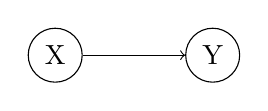
\begin{tikzpicture}
        \node[shape=circle,draw=black] (X) at (0,0) {X};
        \node[shape=circle,draw=black] (Y) at (2,0) {Y};
        \path [->] (X) edge node {} (Y);
    \end{tikzpicture}
\end{center}
\begin{definizione}[\textbf{Condizionalmente indipendente}]
    L'evento $A$ è \textbf{condizionalmente indipendente} dall'evento $B$, se dato
    un evento $C$ vale la seguente relazione:
    \begin{equation}
        P(A|B,C) = P(A|C)
    \end{equation}
    ovvero che la conoscenza a priori di $B$ non influisce sulla probabilità di
    $A$ rispetto a quella che si ha conoscendo $C$.
\end{definizione}
La topologia della rete, ovvero la sua struttura, e le probabilità condizionate
dei nodi dati i loro genitori sono sufficienti a specificare la \textbf{distribuzione
    congiunta} di tutte le variabili rappresentate dalla rete.

La componente quantitativa contenuta in ogni nodo è costituita da un insieme di
\textbf{tabelle di probabilità condizionate} (CPT), queste tabelle rappresentano
l'impatto dei genitori sulla variabile stessa.

Le CPT dicono quant'è la probabilità di assumere un valore per una variabile di
un nodo, condizionata al valore delle variabili dei genitori. L'\textbf{assunzione}
delle reti è che ogni nodo è \textbf{condizionalmente indipendente} dai suoi non
discendenti dati i suoi genitori.

Nella definizione della struttura della rete è importante che il grafo orientato
non contenga cicli, ovvero che la rete Bayesiane sia un DAG (\textit{Directed Acyclic
    Graph}). Questo perché non è possibile che una variabile sia causa di se stessa.
\subsection{Componente Quantitativa}
Consideriamo ora la componente quantitativa di una rete Bayesiane, ovvero le
\textbf{Conditional Probability Tables} (CPT). Di queste tabelle possiamo dire che:
\begin{itemize}
    \item Ogni nodo ha associata una tabella (CPT).
    \item La CPT descrive la probabilità condizionata della variabile dato un
          particolare assegnamento dei valori delle variabili genitore.
    \item La somma di ogni riga della tabella deve essere uguale a $1$.
    \item La CPT di una variabile booleana con $k$ variabili genitori anche essi
          booleani, contiene $2^k$ valori di probabilità che possono essere
          specificati indipendentemente.
    \item Una variabile senza genitori ha una CPT con una sola riga che contiene
          i valori di probabilità a priori per ogni possibile valore che la
          variabile può assumere.
\end{itemize}
\begin{nota}
    Nel caso specifico di variabili booleane, se specifico solo il valore nel
    caso vero nella CPT posso ricavare il valore del caso falso utilizzando:
    \begin{equation*}
        \text{falso} = 1 - \text{vero}
    \end{equation*}
    Quindi il falso è un parametro dipendente.
\end{nota}
Per le reti Bayesiane si può fare sia inferenza \textit{diagnostica}, ovvero fatta
dai figli verso i genitori, sia \textit{prognostica} dai genitori verso i figli.
Posso anche calcolare la probabilità di variabili che non sono in relazione padre
figlio ma che sono connesse.
\section{Semantica delle reti Bayesiane}
La semantica delle reti Bayesiane può essere presentata e compresa in base a:
\begin{itemize}
    \item \textbf{Semantica numerica}: la rete rappresenta una \textbf{distribuzione
              congiunta} di probabilità. Questa invece risulta importante per
          comprendere come sia possibile effettuare inferenza utilizzando la
          probabilità congiunta.
    \item \textbf{Semantica topologica}: la rete codifica un insieme di
          \textbf{relazioni di indipendenza condizionale}. Questa risulta
          importante per comprendere come sia possibile costruire un modello di
          Rete Bayesiane.
\end{itemize}
La costruzione delle reti è un processo incrementale che può essere effettuato
utilizzando le informazioni a priori del dominio se si hanno conoscenze
approfondite di esso, oppure tramite algoritmi di apprendimento.
\subsection{Semantica numerica}
Ogni rete costituisce una descrizione completa del dominio che rappresenta, di
conseguenza la distribuzione congiunta di probabilità di tutte le variabili
rappresentate dalla rete può essere ottenuta direttamente dalla rete stessa.

Un generico elemento della distribuzione di probabilità congiunta è associato a
una realizzazione congiunta delle variabili presenti nella rete.

Ogni elemento della distribuzione di probabilità congiunta può essere calcolato
sfruttando la \textbf{formula di fattorizzazione della distribuzione congiunta}
che è data da:
\begin{equation}
    P(V_1 = v_1,...,V_n = v_n) = \prod_{i=1}^{n} P(V_i=v_i|parents(V_i))
\end{equation}
dove $parents(V_i)$ rappresenta la realizzazione congiunta dei genitori di $V_i$.
Ogni elemento della distribuzione congiunta è rappresentato tramite il prodotto
delle opportune componenti delle CPT dei nodi della rete.
\begin{nota}
    Ricorda che per il teorema di Bayes:
    \begin{equation*}
        P(V_i = v_i|parents(V_i)) = \frac{P(V_i = v_i,parents(V_i))}{P(parents(V_i))}
        = \alpha P(V_i = v_i,parents(V_i))
    \end{equation*}
    Quindi la probabilità condizionata viene considerata come la probabilità
    congiunta divisa per la probabilità degli eventi congiunti. Per semplificare
    la probabilità si può solo calcolare la congiunta e successivamente moltiplicarla
    per il fattore $\alpha$ di normalizzazione.

    Il valore di $\alpha$ per la probabilità $P(V_i=v_i|parents(V_i))$ si trova
    nel seguente modo:
    \begin{equation*}
        \alpha = \frac{1}{P(V_i = \lnot v_i, parents(V_i)) + P(V_i = v_i,parents(V_i))}
    \end{equation*}
\end{nota}
\begin{nota}
    Non si vedono più le dipendenze di una variabile da tutte le altre ma bensì
    probabilità della variabile condizionata dai suoi genitori.
\end{nota}
\subsection{Semantica topologica}
La formula di fattorizzazione implica relazioni di \textbf{indipendenza condizionale}
che possono essere sfruttate per determinare la componente \textbf{topologica}
della rete.

La regola della probabilità congiunta la possiamo scrivere come:
\begin{equation*}
    \begin{aligned}
        P(V_1= v_1,...,V_n = v_n) = P(V_1 = v_1) \cdot P(V_2 = v_2|V_1 = v_1)
        \cdot P(V_3 = v_3|V_1 = v_1,V_2 = v_2) \dots \\
        \dots P(V_n = v_n|V_1 = v_1, \dots,V_{n-1}=v_{n-1}) = \prod_{i=1}^{n}
        P(V_i = v_i| \bigcap_{j = 1}^{i - 1} V_j= v_j)
    \end{aligned}
\end{equation*}
Questa uguaglianza è vera per ogni insieme di variabili aleatorie ed è nota con
il nome di \textbf{chain rule}. Confrontando la formula di fattorizzazione con
la chain rule è possibile verificare che la specificazione della distribuzione
di probabilità congiunta è equivalente all'asserzione generale che per ogni
variabile $v_i$:
\begin{equation}
    P(v_i|v_1,...,v_{i-1}) = P(v_i|parents(v_i))
\end{equation}
a patto che $parents(v_i) \subseteq \{v_1,...,v_{i-1}\}$. Quindi possiamo
considerare la probabilità di $V_i$ condizionata da tutti gli altri nodi della 
rete, può essere vista come la probabilità di $V_i$ condizionata solamente dai 
suoi genitori. Questo ci permette di effettuare una semplificazione molto utile.

Una rete Bayesiane rappresenta correttamente un dominio solo a condizione che ogni
nodo risulti \textbf{condizionalmente indipendente} dai suoi non discendenti
dati i suoi genitori. Pertanto, per costruire una Rete Bayesiana che abbia la
corretta struttura del dominio da modellare è necessario scegliere, per ogni nodo,
i nodi genitore in modo che tale proprietà risulti verificata. In aggiunta un nodo
è \textbf{condizionalmente indipendente} da tutti i nodi restanti della rete data
la conoscenza dello stato del suo \textbf{Markov Blanket}, ovvero l'insieme dei
genitori, dei figli e dei genitori dei figli.
\begin{figure}[!ht]
    \centering
    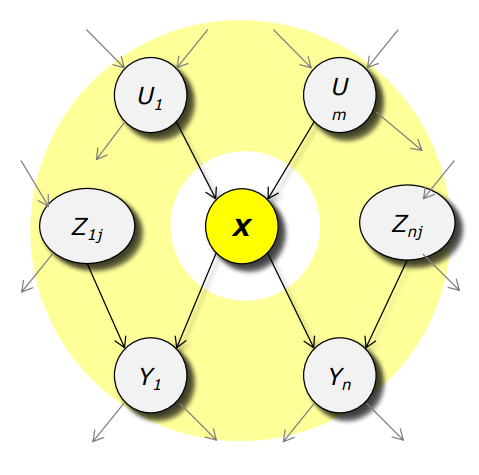
\includegraphics[width=0.5\textwidth]{./img/Reti/MarkovBlanket.png}
    \caption{I nodi $U_i, Z_{ij}, Y_j$ appartengono alla Markov Blanket di $X$}
    \label{fig:MarkovBlanket}
\end{figure}

Una possibile procedura per la costruzione incrementale della componente topologica
di una rete Bayesiane è la seguente:
\begin{itemize}
    \item Scegliere un insieme di variabili $\{x_1, \dots, x_n\}$ che rappresentano
          le variabili del dominio.
    \item Scegliere un ordinamento topologico per le variabili.
    \item Inizializzare il numero dei nodi aggiunti alla rete a $i = 1$.
    \item Selezionare la variabile $X_i$ e aggiungere il nodo corrispondente alla
          rete.
          \begin{itemize}
              \item Porre $parents(X_i)$ uguale all'insieme minimale di nodi,
                    appartenenti alla rete nel momento corrente $\{X_{(1)} \dots X_{(i-1)}\}$
                    che soddisfa la proprietà di indipendenza condizionale.
              \item Computare la CPT per la variabile $X_i$.
          \end{itemize}
    \item Incrementare il numero dei nodi aggiunti alla rete $i=i+1$. E ripetere il
          procedimento per ogni variabile.
\end{itemize}
Il metodo di costruzione delle reti è un passo fondamentale per la corretta
rappresentazione del dominio. La scelta delle relazioni di dipendenza condizionale
impatta notevolmente sulla quantità di parametri che devono essere specificati
per la rete.

Oltre a costituire una rappresentazione completa e non ridondante di un dominio
una Rete Bayesiana è spesso molto più compatta dell'intera distribuzione di
probabilità congiunta. Questo rende possibile il trattamento di domini
caratterizzati da un numero molto elevato di variabili.

La compattezza delle Reti Bayesiane è un esempio della proprietà dei sistemi
strutturati localmente o sparsi. In ogni sistema strutturato localmente ogni
sotto-componente interagisce solo con un numero limitato di altre componenti,
indipendentemente dal numero totale di componenti del sistema.

La strutturazione locale è di norma associata ad un fattore di crescita della
complessità lineare e non esponenziale. Nel caso di una Rete Bayesiana è 
ragionevole ipotizzare che ogni variabile sia direttamente influenzata da al 
massimo $k$ variabili.

Nel caso in cui si consideri una Rete Bayesiana costituita da $n$ variabili
Booleane avremo che la quantità di informazione necessaria per specificare una
qualsiasi CPT è limitata superiormente da $2^k$ numeri per cui la rete completa
richiede di specificare al più $n \cdot 2^k$ numeri. Mentre specificare l'intera
distribuzione congiunta di probabilità richiede $2^n$ numeri.
\subsection{Indipendenza condizionata}
Esiste un metodo per scoprire se in una rete Bayesiana due variabili sono
condizionalmente indipendenti. Questo metodo prende il nome di \textbf{D-separazione}.
\begin{definizione}[\textbf{D-separazione}]
    Due nodi $X$ e $Z$ sono \textbf{D-separati} da un insieme $E$ di variabili con
    evidenza se e solo se ogni cammino non orientato da $X$ a $Z$ è \textbf{bloccato}
\end{definizione}
\begin{definizione}[\textbf{cammino bloccato}]
    Un cammino è \textbf{bloccato} se e solo se vale almeno una delle seguenti
    condizioni:
    \begin{itemize}
        \item Se esiste una variabile $V$ tale che appartiene alle evidenze e
              gli archi del camino sono \textbf{tail-to-tail}.
              \begin{figure}[!ht]
                  \centering
                  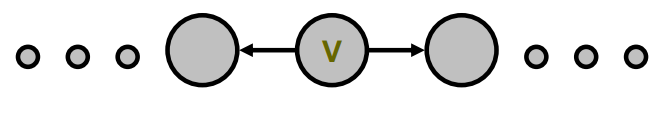
\includegraphics[width=0.5\textwidth]{./img/Reti/TailToTail.png}
                  \caption{Collegamento tail-to-tail}
                  \label{fig:tail-to-tail}
              \end{figure}
        \item Se esiste una variabile $V$ tale che appartiene alle evidenze e
              gli archi che collegano $V$ sono \textbf{tail-to-head}.
              \begin{figure}[!ht]
                  \centering
                  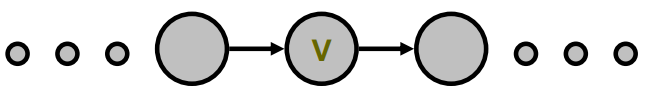
\includegraphics[width=0.5\textwidth]{./img/Reti/TailToHead.png}
                  \caption{Collegamento tail-to-head}
                  \label{fig:tail-to-head}
              \end{figure}
        \item Se esiste una variabile $V$ tale che la variabile e tutti i suoi figli
              \textbf{non} appartengono ad $E$ e gli archi che collegano $V$ al
              resto del cammino sono \textbf{head-to-head}.
              \begin{figure}[!ht]
                  \centering
                  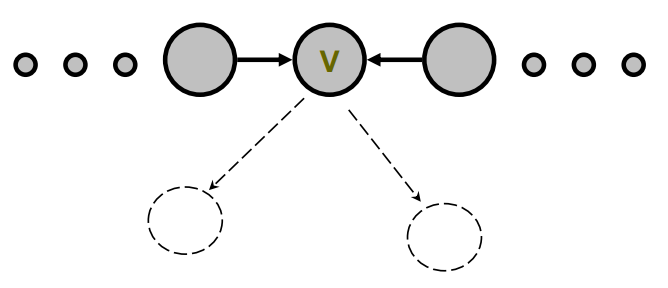
\includegraphics[width=0.5\textwidth]{./img/Reti/HeadToHead.png}
                  \caption{Collegamento head-to-head}
                  \label{fig:head-to-head}
              \end{figure}
    \end{itemize}
\end{definizione}
La d-separazione può essere calcolata in tempo lineare. Quindi abbiamo a
disposizione un algoritmo efficiente per inferire automaticamente se apprendere
il valore di una variabile può fornirci delle informazioni aggiuntive su altre
variabili, date le informazioni a disposizione.
\begin{teorema} [\textbf{Verma \& Pearl}]
    Se in una rete Bayesiana un insieme di variabili $E$ di evidenza D-separa
    $X$ e $Z$, allora $X$ e $Z$ sono indipendenti.
\end{teorema}
\begin{definizione}[\textbf{d-connessione}]
    Due variabili sono \textbf{d-connesse} se e solo se non sono d-separate
\end{definizione}
Per testare se le variabili sono condizionalmente indipendenti si può usare il
\textbf{processo di moralizzazione}:
\begin{enumerate}
    \item \textbf{Disegnare grafo ancestrale}: rete composta delle variabili
          citate e tutti i loro predecessori.
    \item \textbf{Moralizzare il grafo}: per ogni coppia di variabili che hanno
          un figlio in comune, si traccia un arco non orientato tra di loro, in
          caso di più genitori si collegano le coppie a due a due.
    \item \textbf{Disorientiamo il grafo}: sostituzione degli archi orientati
          con archi non orientati
    \item \textbf{Eliminiamo i given e gli archi incidenti}: eliminare i nodi
          facenti parte dell'evidenza e tutte le connessioni.
\end{enumerate}
Se al termine di questo processo si hanno:
\begin{itemize}
    \item \textbf{Variabili disconnesse}: è garantito che le variabili sono
          indipendenti
    \item \textbf{Variabili connesse}: non è garantito che le variabili siano
          indipendenti.
\end{itemize}
\begin{esempio}
    Vediamo ora un esempio del processo di moralizzazione. Vogliamo verificare
    se $A$ e $B$ sono condizionalmente indipendenti dati $D$ e $F$.
    \begin{figure}[!ht]
        \centering
        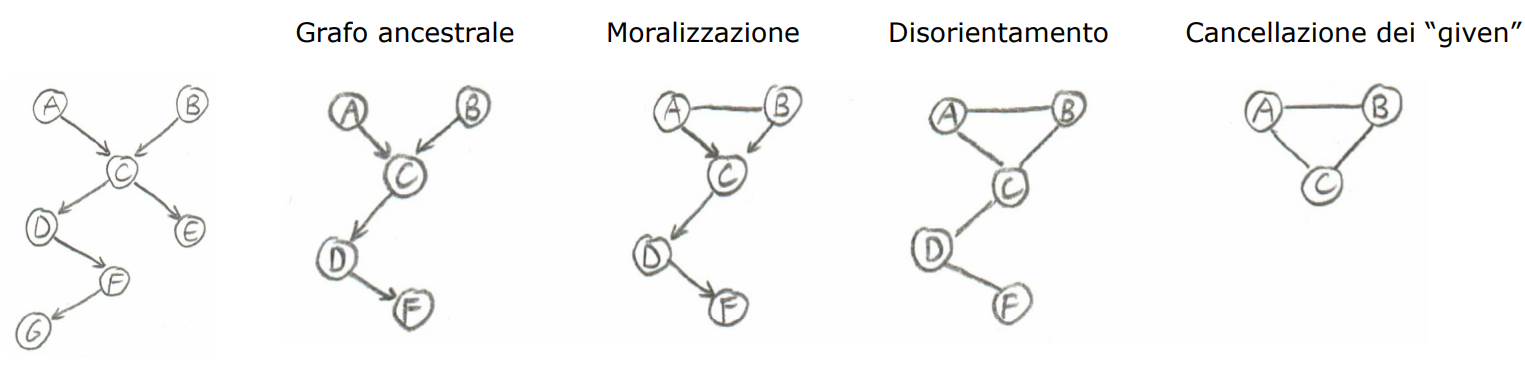
\includegraphics[width=1\textwidth]{./img/Reti/Moralizzazione.png}
        \caption{Esempio di moralizzazione}
        \label{fig:moralizzazione}
    \end{figure}
\end{esempio}
\subsection{Distribuzioni condizionali}
Per ridurre il numero di parametri nelle CPT possiamo utilizzare le \textbf{distribuzioni
    canoniche} per rappresentare dei pattern standard tra i parametri come per
i nodi deterministici. Si possono utilizzare le distribuzioni canoniche solo
quando si possono notare dei pattern particolari, ex: and tra genitori, or tra
genitori, somma dei genitori$\dots$

Una volta identificato il pattern, questo ci permette di specificare un numero 
limitato di parametri per compilare la CPT, dal momento che alcuni si derivano 
con le distribuzioni canoniche.
\begin{definizione}[\textbf{Nodo deterministico}]
    Un \textbf{nodo deterministico} è caratterizzato dal fatto che il valore che
    esso assume è completamente determinato tramite il valore assunto dai suoi
    genitori. Non c'è incertezza.
\end{definizione}
Le relazioni tra genitori e figli possono essere di diversi tipi:
\begin{itemize}
    \item \textbf{Logiche}: come ad esempio l'\texttt{OR} tra le variabili dei genitori.
    \item \textbf{numeriche}: come ad esempio il \texttt{minimo} valore delle
          variabili dei genitori.
\end{itemize}
Un importante pattern è l'\textbf{indipendenza di uno specifico contesto} ovvero
quando la probabilità condizionata di un nodo è condizionalmente indipendente
da alcuni genitori dati certi valori di altri (if-else sintax).

Le relazioni incerte, possono essere caratterizzate dalle \textbf{Noisy Logical
    Relations} che permettono di modellare l'incertezza dei genitori nel causare
il figlio. Queste relazioni sono utili per modellare situazioni in cui la presenza
di un genitore non implica necessariamente la presenza del figlio.
Andiamo per esempio ad analizzare il modello \textbf{Noisy-OR}. Questo modello 
consente di introdurre incertezza circa la capacità di ogni nodo genitore di 
causare il valore vero della variabile figlio. 

Il modello Noisy-OR effettua le seguenti ipotesi:
\begin{itemize}
    \item Tutte le possibili cause sono note
    \item L'inibizione di un genitore è indipendente dall'inibizione degli altri
          genitori per il nodo considerato.
\end{itemize}
In questo caso specifico la probabilità di un determinato evento, è data dal 
prodotto delle probabilità di inibizione per ogni nodo genitore.
\subsection{Rappresentazioni efficiente delle distribuzioni continue}
Per rappresentare efficientemente i nodi di distribuzioni continue, usando quelle
canoniche, possiamo pensare di discretizzare le variabili continue definendo un
insieme finito di intervalli. Il problema che sorge utilizzando questo approccio
è legato alla perdita di informazioni sul dato. Inoltre, le CPT spesso aumentano 
di dimensione.

Una soluzione alternativa è rappresentare le variabili con delle \textbf{funzioni
    di densità di probabilità} vengono descritte tramite un numero finito e di
norma contenuto di parametri. Un esempio è la funzione di densità di probabilità
della distribuzione normale, la quale viene completamente specificata tramite
la media e la deviazione standard.
\begin{definizione}[\textbf{Rete Bayesiana Ibrida}]
    Una rete che contiene nodi discreti e continui prende il nome di \textbf{Rete
        Bayesiane Ibrida}
\end{definizione}
Per specificare una Rete Bayesiana Ibrida dobbiamo definire due nuovi tipi di
distribuzione:
\begin{itemize}
    \item La distribuzione condizionale di una variabile continua dati i genitori
          discreti o continui.
    \item La distribuzione condizionale di una variabile discreta dati i genitori
          continui.
\end{itemize}

\section{Inferenza}
L'obiettivo fondamentale è quello di riuscire a calcolare la posterior di un insieme 
di variabili considerando una serie di variabili di evidenza.

\begin{itemize}
    \item $X$ sarà la variabile di query
    \item $E$ insieme di variabili di evidenza
    \item $e$ specifico evento, ovvero un assegnamento congiunto dei singoli valori
    delle variabili di evidenza
    \item $Y$ insieme di variabili non di evidenza
\end{itemize}

L'insieme complessivo di variabili è $V = \{X\} \cup E \cup Y$. 
Una tipica query della quale bisogna calcolare la posterior è
$$P(X | E = e)$$
Prima chiedevamo di calcolare la distribuzione di probabilità della viabile date 
tutte le altre variabili nella rete.

Nelle reti bayesiane abbiamo diverse tipologia di inferenza:
\begin{itemize}
    \item \textbf{diagnostica}: si passa dagli effetti alle cause, l'evidenza è 
    nei discendenti e l'informormazione sale dai figli ai genitori.
    \item \textbf{causale}: si passa dalle cause agli effetti, l'evidenza è 
    nei genitori e l'informormazione scende dai genitori ai figli.
    \item \textbf{intercausale}: si passa l'informazione tra cause ed effetti comuni
    \item \textbf{mista}: l'informazione è presente sia nel genitore sia nel figlioe 
    quindi abbiamo sia una una componente diagnostica sia una componente intercausale
\end{itemize}

Inserire l'evidenza nella rete allora significa che si devono aggiurnare tutte le 
CPT della rete bayesiana. Quindi implementare il meccanismo inferenza data una 
evidenza allora significa inserire l'evidenza che aggiorna le CPT e successivamente 
si possono evvettuare tutte le query che si vogliono fare. La distribuzione si 
calcola facilmente perché sono state aggiornate precedentemente le CPT in base 
all'evidenza osservata.

% TODO: inserire immagini

Per rispondere ad una query generica 
$$P(X|E=e)$$
allora sfrutto la seguente equazione (algoritmo per enumerazione) 
$$P(X|E=e) = \alpha P(X,E=e) = \alpha \sum_{y} P(X,E=e, Y=y)$$
$\alpha \sum_{y} P(X,E=e, Y=y) \equiv P(X,E=e, Y=y)$ ovvero la probabilità congiunta
tra tutte le variabili, quello che effettivamente calcolavamo precedentemente. 
Si parla di enumerazione perché calcoliamo tutte le possibili combinazioni di valori
delle variabili che non fanno parte dell'evidenza.
Nota che si aggiunge la costante di normalizzazione, ovvero $\alpha = \frac{1}{\prod_{x\in X}^{max}P(X=x)}$.

$P(X,E=e, Y=y)$ la calcoleremo con la regola di fattorizzazione, come facevamo prima.

Quindi in generale 
$$P(X|E=e) = <P(X=x'|E=e), P(X=x''|E=e),\dots>$$

Quindi 
$$P(X=x'|E=e) = \alpha \sum_{y} P(X=x',E=e, Y=y) = \alpha \sum_{y} P(X=x',E=e, Y=y)$$ 
Dove $P(X=x',E=e, Y=y)$ lo calcoliamo come facevamo sempre, ovvero sia $K \in \{X, E, Y\}$
allora 
$$P(X=x',E=e, Y=y) = \prod_{K} P(K=k | parents(K))$$
Mentre $\alpha = \frac{1}{\prod_{x\in X}^{max}P(X=x)}$.

Il processo di inferenza per $n$ variabili booleane è pari a $O(n2^n)$. Possiamo 
migliorare le tempistiche in questo modo:
\begin{itemize}
    \item migliorare il calcolo $P(K=k | parents(K))$ andando a raccogliere 
    quei fattori che non dipendo dalle sommatorie e quindi rispariamo delle moltiplicazioni.
    \item dal momento che calcoliamo tutte le combinazioni dei valori delle variabili
    significa che ricalcoliamo sempre gli stessi valori, quindi cambieremo approccio
    e useremo l'algoritmo delle elimininazioni delle variabili.
\end{itemize}

L'algoritmo si basa sul principio di risolvere il calcolo delle sommatorie in 
\textbf{bottom-up}, ovvero da dx verso sx e si salvano quei valori in modo tale 
da calcolarlo senza ripetizione.

